\subsection{Структура фреймворка}

Для понимания способа изложения методов в дальнейшем, 
следует обсудить разработанную структуру фреймворка.

Для этого
рассмотрим подробнее программную реализацию на примере афинного
шифра, не затрагивая саму реализацию криптоаналитических
функций, которая будет обсуждаться в соответствующем
параграфе.

\vspace{3mm}
\noindent
\parbox[b][8.5cm][t]{10mm}{
    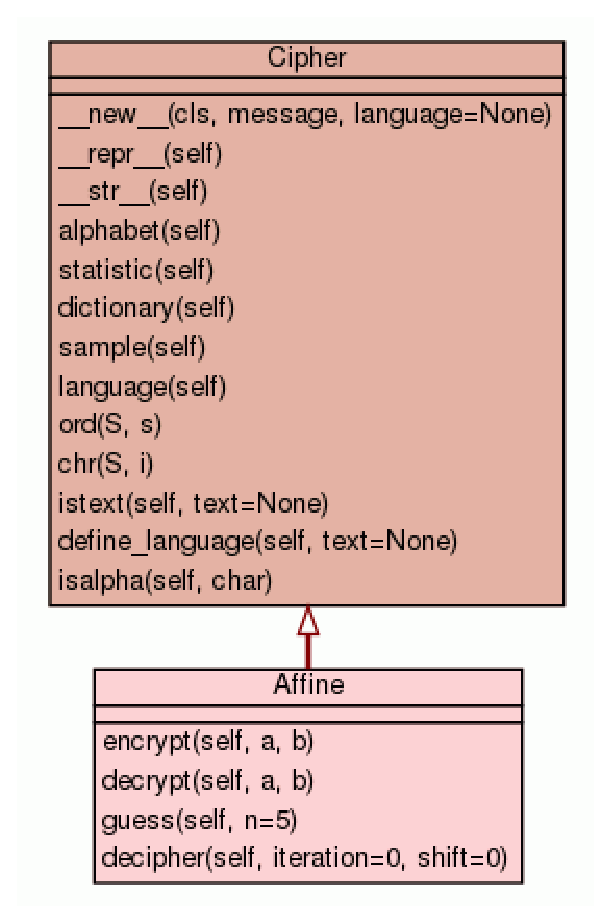
\includegraphics[height=82mm]{\globalImages/uml_affine.eps}
}
\hfill
\parbox[b][8.5cm][t]{107mm}{
    Слева представлена UML диаграмма базового класса \texttt{Cipher} и 
    класса для исследования афинных шифров \texttt{Affine}. Python, выбранный 
    в качестве языка программирования, поддерживает
    парадигму объектно-ориентированного программирования. 

    Базовый класс наследован от класса строки, что позволяет 
    использовать все методы для работы со строками внутри 
    объекта (например, объект шифра можно использовать в 
    итераторе). Соответственно и методы базового класса, 
    необходимые для анализа всех изучаемых шифров будут 
    описаны только в одном месте.

    Первые три метода, название которых начинается и 
    заканчивается двумя подчеркиваниями \_\_ («магические
    методы» в терминологии Python), не вызываются напрямую
    а исполняются при попадании в какой-либо контекст. 
}

Методы 
\texttt{\_\_init\_\_}, \texttt{\_\_repr\_\_} и \texttt{\_\_str\_\_}
управляют созданием, представлением в виде объекта и представлением в виде
строки соответственно.

Оставшиеся методы работают согласно своему названию:

\begin{trivlist}
\item \texttt{alphabet} возвращает алфавит языка;
\item \texttt{statistic} возвращает статистику встречаемости символов в сообщении;
\item \texttt{dictionary} возвращает словарь языка;
\item \texttt{sample} возвращает алфавитные символы в сообщении;
\item \texttt{language} возвращает заданный или определенный язык;
\item \texttt{ord(c)} возвращает позицию символа в алфавите языка;
\item \texttt{chr(n)} возвращает символ на позиции \texttt{n}, то есть \texttt{chr(ord(c)) == c};
\item \texttt{istext(m)} проверяет является ли m осмысленным текстом в языке;
\item \texttt{define\_language(m)} определяет язык сообщения \texttt{m};
\item \texttt{isalpha(c)} проверяет, есть ли символ \texttt{с} в алфавите.
\end{trivlist}

Класс \texttt{Affine} является наследником класса \texttt{Cipher}.
Он реализует три метода, заложенных в родительском классе и 
добавляет свой:

\begin{trivlist}
\item \texttt{encrypt} возвращает зашифрованное сообщение;
\item \texttt{decrypt} возвращает расшифрованное сообщение;
\item \texttt{decipher} возвращает результат криптоанализа (эти три метода 
    технически являются перегруженными методами класса \texttt{Cipher});
\item \texttt{guess} сужает множество ключей расшифровки.
\end{trivlist}

Python не реализует кеширующих свойств для объектов, то есть 
таких свойств, которые рассчитывались бы при первом обращениии
и возвращали бы этот результат при дальнейших обращениях.
Это довольно неудобно в моем случае, так как во время 
исследования некоторых шифрограмм необходимы большие объемы данных 
(например, тетраграммы для выбранного языка). Возможно
расчитывать и подгружать их во время инициализации класса с 
помощью уже обсуждавшегося метода \texttt{\_\_init\_\_}, 
но это будет чувствительно занижать скорость работы 
в случаях где в таких данных нет необходимости.
Такая проблема возникает, например, при анализе 
$n$-грамм: триграммы могут дать достаточно хорошую
оценку для текста и не будет необходимости загружать 
статистику по тетраграммам.

Но такая проблема разрешима с помощью другого механизма
Python --- механизма декораторов.

\DEF\textit{Декоратор} --- это функция, ожидающая другую
функцию в качестве параметра.

Такой подход часто используется в функциональных языках
и был перенесен в Python. Консистентность такой парадигмы 
достигается благодаря тому, что все функции в Python
являются объектами.
В фреймворке используется класс кешиирующих свойств, его
структура представлена на диаграмме \ref{uml_cached}.

\begin{figure}[h]
\noindent\centering{
    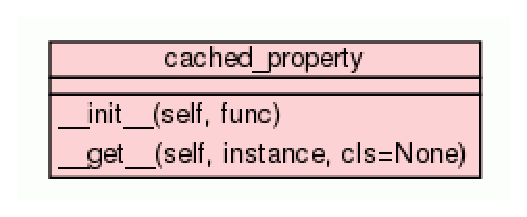
\includegraphics[width=55mm]{\globalImages/uml_cached.eps}
}
\caption{UML диаграмма класса для кеширования свойств}
\label{uml_cached}.
\end{figure}

Использование декоратора:

\begin{listing}[1]{1}
@cached_property
def tetragrams(self):
    '''
    S.tetragrams -> list
    List of tetragrams for selected language.
    '''
    tetragrams = linguistics.get_ngramms(4, self.language)
    return tetragrams
\end{listing}

После первого вызова тетраграммы будут содержаться в 
памяти до выхода из программы.

В итоге, из-за такого структурирования модулей каждый из них
можно использовать как подключаемую библиотеку и как
самодостаточный скрипт.

Пример работы продемонстрирован в IDLE --- это интегрированная среда 
разработки на языке Python, которая позволяет увидеть результат
исполнения сразу после ввода текста.
Работа с классом выглядит так:

\begin{listing}[1]{1}
# ipython3
In [1]: import cipher.classic.affine as a
In [2]: secret = a.Affine('EJJEKI EJ NESR')
In [3]: secret
Out[3]: EJJEK IEJNE SR
In [4]: secret.statistic()
Out[4]: (('E', 4), ('J', 3), ('R', 1), ('S', 1), ('K', 1), ('I', 1), ('N', 1))
In [5]: secret.decipher()
Out[5]: ('ATTACK AT DAWN', 3, 4)
\end{listing}

В первой строке вызывается реализация IDLE, ipython.
В строках со второй по седьмую импортируется модуль
аффинного шифра, создается объект \texttt{secret} с анализируемым
шифротекстом \texttt{EJJEKI EJ NESR}, проверяется работа
вывода и подсчета статистики.
В восьмой строке вызван метод криптоанализа, который
возвращает открытый текст и параметры функции дешифрования 
в девятой строке.

Как уже было сказано,
каждый модуль является исполняемым файлом, для которого
реализован консольный интерфейс по следующей схеме:

\begin{listing}[1]{1}
# ./cipher/classic/affine.py 'EJJEKI EJ NESR'
Analysis...
Defined language is en.
ATTACK AT DAWN
Decryption parametres is a=3 and b=4.

# ./cipher/classic/affine.py -e 9x23 sample/en.opentext > sample/en.affine

# ./cipher/classic/affine.py sample/en.affine 
Analysis...
Defined language is en.
['TO BE, OR NOT TO BE: THAT IS THE QUESTION:', ... 
Decryption parametres is a=9 and b=23.
\end{listing}

В первой строке модуль вызван с помощью ввода параметров из 
командной строки с уже продемонстрированными параметрами.
В строке 7 с параметрами $a$=9 и $b$=23 зашифрован отрывок
соннета Шекспира из файла \texttt{sample/en.opentext},
результат чего записан в файл \texttt{sample/en.affine}.
В девятой строке как аргумент передается только что 
полученный шифротекст и модуль успешно справляется 
с восстановлением открытого текста.

Тепрерь перейем к шифрам и методам их криптоанализа.
